\nopagebreak
\subsection{Затмения}
Диаметр тени спутника при полном центральном затмении (когда центры трёх тел лежат на одной прямой) с большой точностью равен
\begin{equation}
	d_\text{тени} = 2 \cdot \frac{R_{\moon}(a_\oplus - R_\oplus) - R_\odot \left( a_{\moon} - R_\oplus \right)}{a_\oplus - a_{\moon}}.
\end{equation}

\begin{figure}[h!]
    \centering
    \begin{tikzpicture}
        \tkzDefPoint(0, 0){X}
        \tkzDefPoint(-3.5,0){C1}
        \tkzDefShiftPoint[C1](0.5,0){R1}
        
        \def\k{2.5}
        \tkzDefPointBy[homothety=center X  ratio \k](C1) \tkzGetPoint{C2}
        \tkzDefPointBy[homothety=center X  ratio \k](R1) \tkzGetPoint{R2}
        
        \tkzDefLine[tangent from = X](C1,R1) \tkzGetPoints{A1}{B1}
        \tkzDefLine[tangent from = X](C2,R2) \tkzGetPoints{A2}{B2}
        
        \tkzDrawPolygon[fill=gray!40,draw=none](X,A1,B1)
        
        \tkzDrawCircles[fill=white, thick, draw=black](C1,R1 C2,R2)
        \tkzDrawSegments(X,A2 X,B2 X,C2 C2,A2 C2,B2 C1,A1 C1,B1)
        
        \tkzLabelSegments[left=-1pt](C2,B2 C2,A2){$R$}
        \tkzLabelSegments[left=-2pt](C1,B1 C1,A1){$r$}
        \tkzLabelSegment[above=-1.5pt](C1,C2){$d$}
        \tkzLabelSegment[above=-1.5pt](C1,X){$x$}
        
        \tkzMarkRightAngles[size=0.15](C2,A2,X X,B2,C2 C1,A1,X X,B1,C1)
        \tkzDrawPoints(C1, C2, A1, A2, B1, B2, X)
    \end{tikzpicture}
    \caption{\change{Схема построение тени}}
    \label{pic:shadow-length}
\end{figure}

\begin{figure}[h!]
    \centering
    \begin{tikzpicture}
        \tkzDefPoint(0, 0){X}
        \tkzDefPoint(-3.5,0){C1}
        \tkzDefShiftPoint[C1](0.7,0){R1}
        \tkzDefPoint(-0.5,0){C3}
        \tkzDefShiftPoint[C3](-1,0){R3}
        
        \def\k{2.5}
        \tkzDefPointBy[homothety=center X  ratio \k](C1) \tkzGetPoint{C2}
        \tkzDefPointBy[homothety=center X  ratio \k](R1) \tkzGetPoint{R2}
        
        \tkzDefLine[tangent from = X](C1,R1) \tkzGetPoints{A1}{B1}
        \tkzDefLine[tangent from = X](C2,R2) \tkzGetPoints{A2}{B2}
        
        \tkzInterLC(X,B1)(C3,R3)  \tkzGetPoints{x}{H1}
        \tkzInterLC(X,A1)(C3,R3)  \tkzGetPoints{H2}{x}
        
        \tkzDrawPolygon[fill=gray!40,draw=none](X,A1,B1)
        
        
        \tkzDrawCircles[fill=white, thick, draw=black](C1,R1 C2,R2 C3,R3)
        \tkzDrawSegments(H2,A2 H1,B2 R3,C2 C2,A2 C2,B2 C1,A1 C1,B1)
        \tkzDrawSegments[dashed](H2,X H1,X R3,X)
        
        \begin{scope}[
            dim style/.style={black, latex-latex, opacity=1},
            dim fence style/.style={black, opacity=1}
        ]
            \tkzDrawSegment[opacity=0, dim={$R$, -1.1cm, above=2pt}](C3,R3)
            \tkzDrawSegment[opacity=0, dim={$d_2$, -1.5cm, above=2pt}](C3,C1)
            \tkzDrawSegment[opacity=0, dim={$d_1$, -2cm, above=2pt}](C3,C2)
            \tkzDrawSegment[opacity=0, dim={$h$, 1.1cm, below=2pt}](X,R3)
            \tkzDrawSegment[opacity=0, dim={$x$, 1.5cm, above=2pt}](X,C1)
        \end{scope}
        
        \tkzLabelSegments[right=-1pt](C2,B2 C2,A2){$R_0$}
        \tkzLabelSegments[right=-2pt](C1,B1 C1,A1){$r$}
        \tkzLabelSegments[left=-2pt](R3,H1 R3,H2){$s$}
        
        \tkzMarkRightAngles[size=0.15](C2,A2,X X,B2,C2 C1,A1,X X,B1,C1)
        \tkzDrawPoints(C1, C2, A1, A2, B1, B2, X, C3, R3, H1, H2)
    \end{tikzpicture}
    \caption{\change{К вычислению диаметра пятна}}
    \label{pic:shadow-size-on-surface}    
\end{figure}


Среднее значение  этой величины около 200~км, максимальное~--- около 215~км. При нецентральном затмении максимальный диаметр тени Луны на поверхности Земли может достигать 270~км. Это даёт оценку на продолжительность, равную 7.5 минутам. Большинство полных затмений длятся 2\,--\,4~минуты.

\begin{figure}[h!]
	\centering
	\vspace{-.5pc}
	\begin{tikzpicture}[xscale=1.2]
            
        \tkzInit[
            xmax=1,
            xmin=-7,
            ymin=-1.2,
            ymax=1.2
        ]
        \tkzClip    
            
        \def\e{0}
        \def\m{-1.3}
        \def\s{-6}
        
        \def\earthR{0.7}
        \def\moonR{0.18}
        \def\sunR{1}
        
        \tkzDefPoint(\e,0){E}
        \tkzDefPoint(\m,0){M}
        \tkzDefPoint(\s,0){S}
        
        
        
        \tkzDefShiftPoint[S](0,\sunR){S'}
        \tkzDefShiftPoint[M](0,\moonR){M'}
        \tkzDefShiftPoint[E](0,\earthR){E'}
        
        \def\shadeCornerCoef{\sunR / (\sunR - \moonR)}
        \tkzDefPointBy[homothety=center S ratio \shadeCornerCoef](M)
        \tkzGetPoint{SC}
        
        \def\halfShadowCornerCoef{\sunR / (\sunR + \moonR)}
        \tkzDefPointBy[homothety=center S ratio \halfShadowCornerCoef](M)
        \tkzGetPoint{HSC}
        
        \tkzDefLine[tangent from = SC](S,S')  \tkzGetPoints{S1}{S2}
        \tkzDefLine[tangent from = SC](M,M')  \tkzGetPoints{M1}{M2}
        \tkzDefLine[tangent from = HSC](S,S')  \tkzGetPoints{HS1}{HS2}
        \tkzDefLine[tangent from = HSC](M,M')  \tkzGetPoints{HM1}{HM2}
        
        \tkzInterLC(SC,S1)(E,E') \tkzGetSecondPoint{E1}
        \tkzInterLC(SC,S2)(E,E') \tkzGetFirstPoint{E2}
        
        \tkzGetVectxy(HSC,M){hs}
        \def\halfShadowCoef{(\e - \m + \hsx) / \hsx }
        \tkzDefPointBy[homothety=center HSC ratio \halfShadowCoef](HM1)
        \tkzGetPoint{HE1}
        \tkzDefPointBy[homothety=center HSC ratio \halfShadowCoef](HM2)
        \tkzGetPoint{HE2}
        
        
        \tkzDrawSector[fill=gray!30,gray!30](HSC,HE2)(HE1)
        \tkzDrawSector[fill=gray!70](SC,M2)(M1)
        \tkzDrawSector[fill=white](HSC,HM2)(HM1)
        
        \tkzDrawCircles[dashed, line width=.4pt](S,E E,M) 

        \tkzDrawCircles[black, line width=.4pt, fill=white](S,S' M,M')
        \tkzDrawSegments(SC,S1 SC,S2 HS1,HE1 HS2,HE2)
%        \tkzDrawSegments(S,S1 S,S2 S,HS1 S,HS2 M,M1 M,M2 M,HM1 M,HM2)
%        \tkzDrawPoints(S1, S2, SC, HS1, HS2, M1, M2, HM1, HM2)
        
        \tkzDrawCircles[black, line width=.4pt, fill=white, fill opacity=1](E,E')
%        \tkzDrawPoints(E1, E2)
        
        \tkzLabelPoint[inner sep=5mm](S){\tikz{\sun(S)}}
        \tkzLabelPoint(E){\tikz{\earth(E)}}
        \tkzLabelPoint(M){$\rightmoon$}
    \end{tikzpicture}
	\caption{Полное солнечное затмение со стороны северного полюса эклиптики}
	\label{fig:eclipses-full-solar-eslipse}
\end{figure}
При \term[кольцеобразное солнечное затмение]{кольцеобразном солнечном затмении} Луна так расположена относительно Земли, что конус её тени не достаёт до поверхности планеты, и вокруг Луны можно наблюдать яркое кольцо незакрытой части солнечного диска.

\begin{figure}[h!]
	\centering
	\begin{tikzpicture}[xscale=1.2]
	
	    \tkzInit[
            xmax=1,
            xmin=-7,
            ymin=-1.2,
            ymax=1.2
        ]
        \tkzClip
            
        \def\e{0}
        \def\m{-1.8}
        \def\s{-6}
        
        \def\earthR{0.7}
        \def\moonR{0.18}
        \def\sunR{1}
        
        \tkzDefPoint(\e,0){E}
        \tkzDefPoint(\m,0){M}
        \tkzDefPoint(\s,0){S}
        
        
        \tkzDefShiftPoint[S](0,\sunR){S'}
        \tkzDefShiftPoint[M](0,\moonR){M'}
        \tkzDefShiftPoint[E](0,\earthR){E'}
        
        \def\shadeCornerCoef{\sunR / (\sunR - \moonR)}
        \tkzDefPointBy[homothety=center S ratio \shadeCornerCoef](M)
        \tkzGetPoint{SC}
        
        \def\halfShadowCornerCoef{\sunR / (\sunR + \moonR)}
        \tkzDefPointBy[homothety=center S ratio \halfShadowCornerCoef](M)
        \tkzGetPoint{HSC}
        
        \tkzDefLine[tangent from = SC](S,S')  \tkzGetPoints{S1}{S2}
        \tkzDefLine[tangent from = SC](M,M')  \tkzGetPoints{M1}{M2}
        \tkzDefLine[tangent from = HSC](S,S')  \tkzGetPoints{HS1}{HS2}
        \tkzDefLine[tangent from = HSC](M,M')  \tkzGetPoints{HM1}{HM2}
        
        \tkzInterLC(SC,S1)(E,E') \tkzGetSecondPoint{E1}
        \tkzInterLC(SC,S2)(E,E') \tkzGetFirstPoint{E2}
        
        \tkzGetVectxy(HSC,M){hs}
        \def\halfShadowCoef{(\e - \m + \hsx) / \hsx }
        \tkzDefPointBy[homothety=center HSC ratio \halfShadowCoef](HM1)
        \tkzGetPoint{HE1}
        \tkzDefPointBy[homothety=center HSC ratio \halfShadowCoef](HM2)
        \tkzGetPoint{HE2}
        
        \tkzDefPointBy[homothety=center SC ratio -1](M1) \tkzGetPoint{SC1}
        \tkzDefPointBy[homothety=center SC ratio -1](M2) \tkzGetPoint{SC2}
        
        \tkzDrawSector[fill=gray!30,gray!30](HSC,HE2)(HE1)
        \tkzDrawSector[fill=gray!70](SC,M2)(M1)
        \tkzDrawSector[fill=gray!50](SC,SC2)(SC1)
        \tkzDrawSector[fill=white](HSC,HM2)(HM1)

        \tkzDrawCircles[dashed, line width=.4pt](S,E E,M) 

        \tkzDrawCircles[black, line width=.4pt, fill=white](S,S' M,M')
        \tkzDrawSegments(SC,S1 SC,S2 HS1,HE1 HS2,HE2)
%        \tkzDrawSegments(S,S1 S,S2 S,HS1 S,HS2 M,M1 M,M2 M,HM1 M,HM2)
%        \tkzDrawPoints(S1, S2, SC, HS1, HS2, M1, M2, HM1, HM2)
        
        \tkzDrawCircles[black, line width=.4pt, fill=white, fill opacity=1](E,E')
%        \tkzDrawPoints(E1, E2)
        
        \tkzLabelPoint[inner sep=5mm](S){\tikz{\sun(S)}}
        \tkzLabelPoint(E){\tikz{\earth(E)}}
        \tkzLabelPoint(M){$\rightmoon$}
    \end{tikzpicture}
%	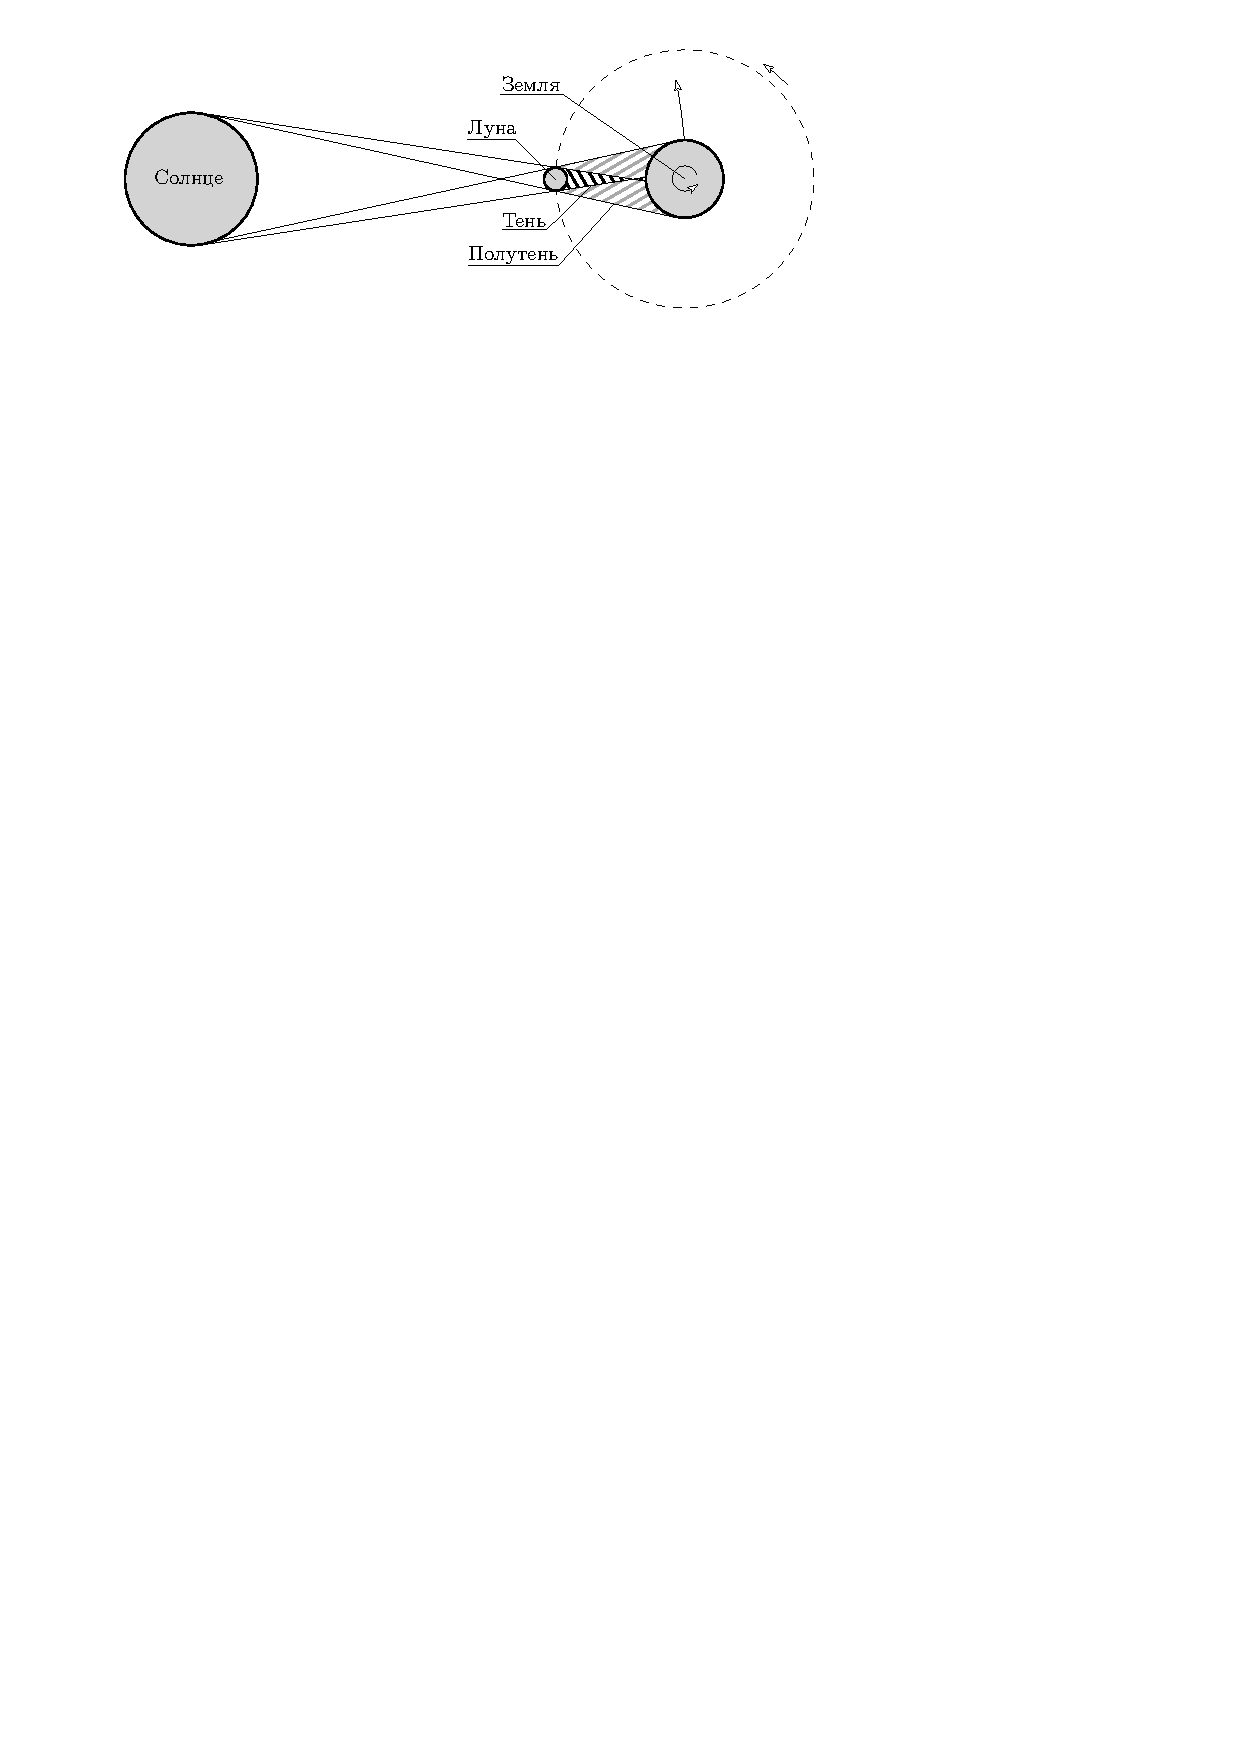
\includegraphics[width = 10cm]{partly-eclipse}
	\caption{Кольцеобразное солнечное затмение со стороны северного полюса эклиптики}
	\label{fig:eclipses-circle-solar-eslipse}
\end{figure}
При особом расположении Луны и Земли возможны \term{гибридные} затмения, когда в разных пунктах Земли наблюдаются либо \imp{кольцеобразное}, либо \imp{полное} затмение. Причиной такого явления является шарообразность Земли.

\vspace{-1pc}
\begin{figure}[h!]
	\centering
	\begin{tikzpicture}[xscale=1.2]
            
        \tkzInit[
            xmax=2.2,
            xmin=-7,
            ymin=-1.2,
            ymax=1.2
        ]
        \tkzClip
            
        \def\e{1.8}
        \def\m{0}
        \def\s{-6}
        
        \def\earthR{0.25}
        \def\moonR{0.7}
        \def\sunR{1}
        
        \tkzDefPoint(\e,0){E}
        \tkzDefPoint(\m,0){M}
        \tkzDefPoint(\s,0){S}
        
        
        \tkzDefShiftPoint[S](0,\sunR){S'}
        \tkzDefShiftPoint[M](0,\moonR){M'}
        \tkzDefShiftPoint[E](0,\earthR){E'}
        
        \def\shadeCornerCoef{\sunR / (\sunR - \moonR)}
        \tkzDefPointBy[homothety=center S ratio \shadeCornerCoef](M)
        \tkzGetPoint{SC}
        
        \def\halfShadowCornerCoef{\sunR / (\sunR + \moonR)}
        \tkzDefPointBy[homothety=center S ratio \halfShadowCornerCoef](M)
        \tkzGetPoint{HSC}
        
        \tkzDefLine[tangent from = SC](S,S')  \tkzGetPoints{S1}{S2}
        \tkzDefLine[tangent from = SC](M,M')  \tkzGetPoints{M1}{M2}
        \tkzDefLine[tangent from = HSC](S,S')  \tkzGetPoints{HS1}{HS2}
        \tkzDefLine[tangent from = HSC](M,M')  \tkzGetPoints{HM1}{HM2}
        
%        \tkzInterLC(SC,S1)(E,E') \tkzGetSecondPoint{E1}
%        \tkzInterLC(SC,S2)(E,E') \tkzGetFirstPoint{E2}
        
        \tkzGetVectxy(HSC,M){hs}
        \def\halfShadowCoef{1 + (\e - \m + \hsx) / \hsx }
        \tkzDefPointBy[homothety=center HSC ratio \halfShadowCoef](HM1)
        \tkzGetPoint{HE1}
        \tkzDefPointBy[homothety=center HSC ratio \halfShadowCoef](HM2)
        \tkzGetPoint{HE2}
        
        
        \tkzDrawSector[fill=gray!30,gray!30](HSC,HE2)(HE1)
        \tkzDrawSector[fill=gray!70](SC,M2)(M1)
        \tkzDrawSector[fill=white](HSC,HM2)(HM1)
        
        
        \tkzDrawCircles[dashed, line width=.4pt](S,M M,E)

        \tkzDrawCircles[black, line width=.4pt, fill=white](S,S' M,M')
        \tkzDrawSegments(SC,S1 SC,S2 HS1,HE1 HS2,HE2)
%        \tkzDrawSegments(S,S1 S,S2 S,HS1 S,HS2 M,M1 M,M2 M,HM1 M,HM2)
%        \tkzDrawPoints(S1, S2, SC, HS1, HS2, M1, M2, HM1, HM2)
        
        \tkzDrawCircles[black, line width=.4pt, fill=white, fill opacity=1](E,E')
%        \tkzDrawPoints(E1, E2)
        
        \tkzLabelPoint[inner sep=5mm](S){\tikz{\sun(S)}}
        \tkzLabelPoint(M){\tikz{\earth(E)}}
        \tkzLabelPoint(E){$\rightmoon$}
    \end{tikzpicture}
%	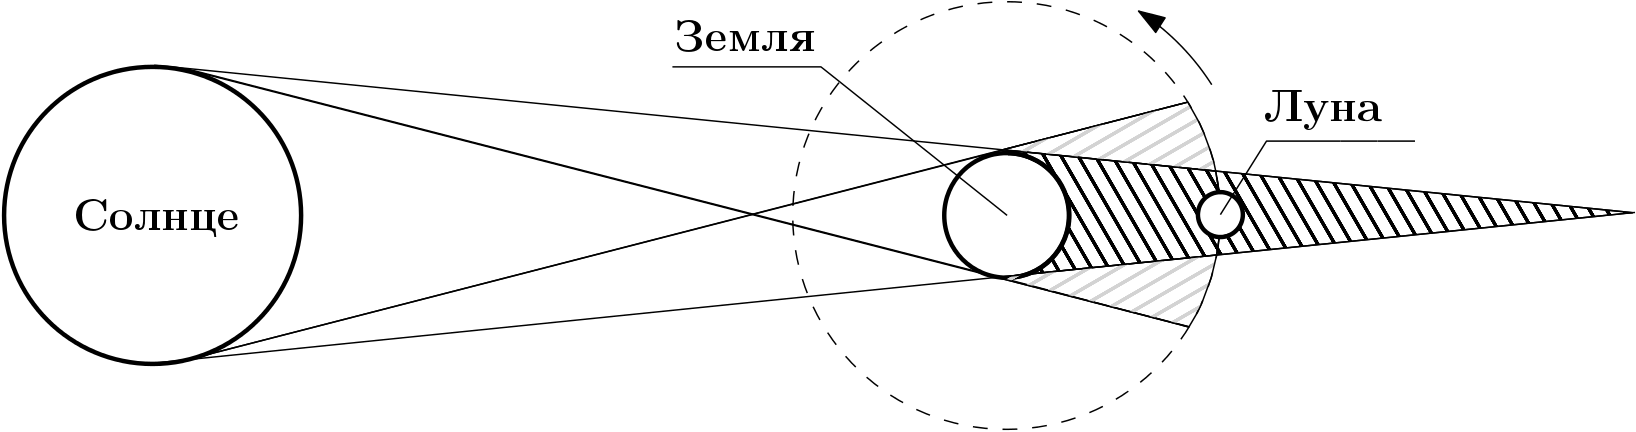
\includegraphics[width=10cm]{moon-eclipse}
	\caption{Схема лунного затмения со стороны северного полюса эклиптики}
	\label{fig:moon-eclipse-scheme}
\end{figure}
\term{Лунное затмение}, в отличие от солнечного, видно со всего ночного полушария Земли. Диаметр земной тени на расстоянии Луны превышает размер последней примерно в 2.5\,--\,3 раза. Бывают \term[частное затмение]{частные}, когда лишь часть Луны попадает в земную тень, \term[полное затмение]{полные}~--- Луна полностью погружается в тень Земли, и \term[полутеневое затмение]{полутеневые}~--- Луна проходит через полутень Земли, не затрагивая конус тени.

\term{Синодический месяц}~--- промежуток времени между одинаковыми фазами Луны, равен 29.53 суток.

\term{Драконический месяц}~--- промежуток времени между двумя последовательными прохождениями Луны через один и тот же узел орбиты,~--- 27.21 суток.

\term{Сарос}~--- промежуток  времени, по прошествии которого солнечные и лунные затмения повторяются в прежнем порядке. Происходит это из-за того, что каждый сарос Луна, орбита Луны и Солнце возвращаются в прежнее положение относительно далёких звёзд. Сарос длится ровно 242 драконических месяца, или 223 синодических месяца, или 18 лет 11 дней 8 часов.

\begin{wrapfigure}[8]{r}{.42\tw}
	\centering
	\vspace{-1pc}
	\includegraphics[width = 0.2\textwidth]{phases}
	\hfill
	\includegraphics[width = 0.2\textwidth]{phases-2}
	\caption{Частное и полное затмение}
	\label{fig:part-eclipses-scheme}
\end{wrapfigure}
Важной характеристикой любого затмения является его \term{фаза}~--- для \imp{частных} и \imp{кольцеобразных} затмений: отношение закрытой части $x$ диаметра\footnote{Здесь имеется в виду \imp{угловой} диаметр} затмеваемого тела, проходящего через центр затмевающего тела, ко всему диаметру затмеваемого тела $D$; для \imp{полного}: единица плюс отношение расстояния\footnote{Расстояние между окружностями $l_1$ и $l_2$~--- это $\min |L_1L_2|$ по всем $L_1 \in l_1$ и $L_2 \in l_2$.} между краями дисков затмеваемого и затмевающего тел к диаметру затмеваемого тела $D$.
\begin{equation}
	\Phi_{\text{част}} = \frac{x}{D} < 1, \quad \quad \quad \Phi_{\text{полн}} =  1 + \frac{\min\{d_1, d_2\}}{D} > 1.
\end{equation}
Иногда вводят такое понятие, как \term{площадная фаза затмения}, т.\,е. отношение площади закрытой части диска затмеваемого тела к полной площади его диска. Чаще всего  площадную фазу используют применительно к двойным звёздам, когда считают падение блеска при затмении одной звезды другой.
